\documentclass[oneside, final, 14pt]{report}
\usepackage[utf8]{inputenc}
\usepackage[russianb]{babel}
\usepackage{vmargin}
\setpapersize{A4}
\setmarginsrb{1cm}{1cm}{1cm}{1.5cm}{0pt}{0mm}{0pt}{13mm}
\usepackage{graphics}
\usepackage[pdftex]{graphicx}
\usepackage{subfigure}
\usepackage{float} %"Плавающие" картинки
\usepackage{wrapfig} %Обтекание фигур (таблиц, картинок и прочего)
\usepackage{amsmath}
\usepackage{moreverb}
\usepackage{indentfirst}
\sloppy

\begin{document}
\Large
\centerline{Бюджетное учреждение высшего образования}
\vskip1.0mm
\centerline{Ханты-Мансийского автономного округа --- Югры}   
\centerline{"<СУРГУТСКИЙ ГОСУДАРСТВЕННЫЙ УНИВЕРСИТЕТ">}
\vskip8mm
\centerline{Политехнический институт}
\centerline{\hfill\hrulefill\hrulefill\hfill}
\vskip1mm
\centerline{Кафедра прикладной математики}
\vskip1cm
\centerline{РАССАДИН АЛЕКСАНДР АНДРЕЕВИЧ}
\vskip1cm
\centerline{Дисциплина "<Уравнения математической физики">}
\vskip3cm
\centerline{ОТЧЁТ}
\centerline{Индивидуальное задание №1}
\begin{center}
Тема "<Численное решение начально-краевых задач для одномерного уравнения теплопроводности">
\end{center}
\vfill
\rightline{Студент гр. №\underline{601-01}} %
\rightline{Рассадин А.А} %
\begin{flushright}

 \rule{5cm}{0.1mm}
\end{flushright}
\vskip1cm
\rightline{Преподаватель} %
\rightline{Гореликов А.В} %
\begin{flushright}
 \rule{5cm}{0.1mm}
\end{flushright}
\centerline{Сургут 2022г.}
\newpage
\Large
\tableofcontents
\chapter{Введение}
На сегодняшний день благодаря техническому прогрессу и развитию точных наук люди научились описывать много вещей, происходящих в мире. В основе этих описаний лежат математические модели. В последнее время математическое моделирование широко используется во многих сферах человеческой деятельности. Оно позволяет достигать высоких показателей в промышленности, экономить природные и денежные ресурсы.

С другой стороны, нельзя недооценивать сложность правильного применения моделирования. Человек, занимающийся этим родом деятельности должен хорошо знать предметную область, обладать соответствующей математической подготовкой. Обязательным этапом при практическом применении компьютерного моделирования является расчёт модели. Следовательно, нужно знать устройство и особенности современных компьютеров и вычислительных систем. Наконец, важно владеть большим числом различных методов для того, чтобы в зависимости от характера задачи выбирать наилучший из них. 

Нужно сказать, что моделирование это очень широкое понятие. Если рассматривать только математическое моделирование, то и в этой отрасли можно выделить ещё несколько разных сфер. К ним относятся: теоретические исследования --- создание новых моделей, методы решения задач --- разработка новых способов решения, а также правильная обработка результатов вычислений. 

Данная работа относится к сфере методов решения задач, точнее к численному решению дифференциальных уравнений в частных производных. С помощью таких уравнений описывается множество явлений в физике и химии. Однако среди этих уравнений есть много таких, которые \emph{невозможно решить аналитически}, поэтому применяют \emph{численный} метод. Такие методы основаны на проведении многократных расчётов. Современные ЭВМ дают много возможностей для применения этих методов, поэтому они активно развиваются. Одним из таких методов --- является метод контрольного объёма\footnote{Часто в тексте он будет записан кратко как "<МКО">.}. Будет показано, как он применяется при численном решении одной из классических задач: задаче о распространении тепла в тонком стержне. В результате будет создана программа, способная рассчитать распределение температуры в стержне с течением времени в зависимости от заданных условий. Результаты расчётов будут представлены в удобном для восприятия формате: в виде анимации. Основным критерием при тестировании должно быть соответствие точности данных, полученных программой с теоретической оценкой.   
\section{Постановка задачи}
Главная цель данной работы --- приобретение первичных навыков математического моделирования, а также получение первого опыта моделирования на основе этих знаний. Требуется изучить математическую модель переноса тепла в твёрдом теле. Ознакомиться с методом контрольных объёмов --- одним из способов численного решения задач такого вида. Затем выполнить реализацию этого метода в виде расчётной программы. При разработке программы нужно сделать так, чтобы её выходные данные потом можно было визуализировать. На финальном этапе должно быть сделано тестирование созданной программы. 
\chapter{Математическая модель}
\section{Уравнение теплопроводности}
Много физических явлений описываются с помощью дифференциальных уравнений с заданными дополнительными условиями. В этой части будет рассмотрено уравнение, которое описывает теплопроводность в твёрдом теле. Рассматривается простейший случай, когда тело это достаточно тонкий\footnote{Предполагается, что в пределах поперечного сечения температура одинакова.} стержень. Уравнение теплопроводности в этом случае имеет следующий вид: 
\begin{equation}
\rho c\frac{\partial U(x,t)}{\partial t} \ = \ \frac{\partial}{\partial x}(k\frac{\partial U(x,t)}{\partial x}) \ + \ f(x,t) \label{eq_HeatTransEq} 
\end{equation}

Оно является частным случай общего уравнения для трёхмерного тела. Подробный вывод общего уравнения можно найти в \cite{bib:UMF_lectures}. Здесь $\rho $ --- плотность материала, из которого сделан стержень, $c$ --- удельная теплоёмкость, $k$ --- коэффициент теплопроводности (на сколько быстро тело способно менять температуру). $U$ --- искомая величина, зависящая от двух значений $x$ и $t$, $f(x, t)$ - плотность тепловых источников\footnote{Плотность тепловых источников --- количество теплоты выделяемой/поглощаемой в единице объёма за 1 секунду.}, величина $T$ --- конечное время наблюдений. Коэффициенты $\rho, c, k$ - записаны как константы, но на самом деле в реальных процессах бывает так, что и плотность $\rho$, и удельная теплоёмкость $c$, и коэффициент теплопроводности $k$ могут быть функциями от $x,\ t$ или даже $U$, или вдобавок зависеть от температуры $U$. Примером такой ситуации может быть стержень, у которого части сделаны из разных материалов, в нём $k$ принимает значения зависящие от положения в стержне, то есть $k \ = \ k(x)$. В данной работе будет предполагаться, что $\rho,\ c,\ k$ - постоянные величины.


Под решением уравнения (\ref{eq_HeatTransEq}) понимается функция $U(x, t)$, которая при подстановке её в уравнение (\ref{eq_HeatTransEq}) обращает его в тождество на заданном множестве изменения переменных $x, t$. В данной задаче это множество $x \in (0, l), \ t \in (0, T]$. Функция $U(x, t)$ описывает значение температуры стержня в точке $x$ в момент времени $t$

\begin{figure}[t!]
    \centering
    \scalebox{1.2}[1]{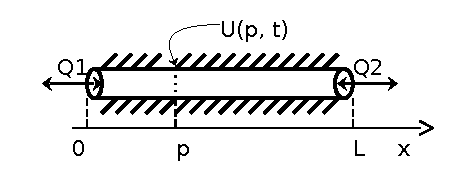
\includegraphics{../img_pdf_cropped/boundary_streams}}
    \caption{$Q_1, \ Q_2$ показывают тепловые потоки на концах стержня. Штрихи обозначают, что через боковую поверхность теплообмена нет.}
    \label{img_boarder_streams}
\end{figure}

Уравнение (\ref{eq_HeatTransEq}) получено из фундаментального закона: закона сохранения энергии. Его левая часть отражает изменение тепловой энергии тела. А слагаемые справа описывают факторы, которые вызывают это изменение. Первое из них возникает из-за теплообмена с внешней средой, который происходит благодаря диффузии, когда сталкиваются молекулы разных скоростей. Второе слагаемое --- так называемый источниковый член. Он отражает вклад от внутренних источников/поглощателей тепла в теле. Всякая математическая модель учитывает лишь часть свойств объекта или явления. Поэтому говорят, что у модели есть \emph{границы применимости}. В случае одномерного уравнения теплопроводности (\ref{eq_HeatTransEq}) можно говорить о неточности данной модели. В том смысле, что учитывается лишь теплообмен через концы стержня\footnote{Если учесть теплообмен ещё и через боковую поверхность, то в уравнении появится дополнительное слагаемое, содержащее искомую величину $U(x, t)$.}, а вся боковая поверхность считается теплоизолированной. Это показано на рис.~\ref{img_boarder_streams}. 


Если для уравнения (\ref{eq_HeatTransEq}) существует решение $U(x, t)$, то ему в этом случае будет также удовлетворять и функция $U(x, t) + C$, где $C$ --- \emph{произвольное} постоянное число. Таким образом, дифференциальное уравнение либо не имеет решений, либо их \emph{бесконечное} число.
В математической модели присутствуют кроме уравнений, также и дополнительные условия. С математической точки зрения они нужны, чтобы уравнением (\ref{eq_HeatTransEq}) функция $U(x, t)$ определялась \emph{однозначно}. 
\section{Дополнительные условия}
В разных математических моделях дополнительные условия могут отличаться. Для случая с явлением переноса тепла в твёрдом теле
нужно задать \emph{начальные} и \emph{граничные} условия. 


Начальные условия означают, что известно распределение температуры во всем теле в начальный момент времени и задаются таким образом:
\begin{equation}
U(x,t_0) = \varphi(x), \quad x \in [0; l] \label{eq_SstartCond}                              
\end{equation}

Аналитически это распределение ~выражается функцией $\varphi(x)$. В дальнейшем всегда будет предполагаться, что $t_0 = 0$. Если $\varphi(x) \equiv 0$, то принято нулевые начальные условия называть \emph{однородными}. 


Кроме распределения температуры в начальный момент времени, для однозначного определения функции $U(x,t)$ нужно также задать граничные условия (ГУ) протекания процесса. То есть выражения, которые описывают температуру или тепловой поток.\footnote{Тепловой поток --- физическая величина, численно равная количеству теплоты проходящей через единичную площадку за одну секунду.} на границе исследуемой области в течение всего эксперимента. 
\newpageОбщий вид граничных условий в одномерном случае такой: 
\begin{equation}
 \alpha(p)\frac{\partial U(p,t)}{\partial x} \ + \ \beta(p)U(p, t) \ = \ \psi(p, t) \label{eq_boundaryCond}
\end{equation}

Точка $p$ пробегает множество граничных точек, а $t > 0$. В данном случае граница области состоит из вдух точек - левого и правого концов стержня. $p \in \{0\}\cup\{l\}$. Производная в уравнении понимается к \emph{односторонняя}. В зависимости от значений $\alpha(p), \ \beta(p)$. Выделяют особого три частных случая: 
\begin{itemize}
 \item $\alpha(p) \equiv 0$ --- первый род, когда известна температура границы (задача Дирихле)
 \item $\beta(p) \equiv 0$ --- второй род ГУ, когда задан тепловой поток (задача Неймана)
 \item $\alpha(p) \neq0$ и $\beta(p) \neq0$ --- третий род ГУ, теплообмен через границу происходит по закону Ньютона-Рихмана (задача Робена)
\end{itemize}


Также как и в случае с нулевыми начальными условиями, когда выделяют случай однородных граничных условий. 
Математически доказано, что для уравнения (\ref{eq_HeatTransEq}) с начальными условиями (\ref{eq_SstartCond}) и граничными условиями (\ref{eq_boundaryCond}), в случае существования решения, оно будет \emph{единственным}. Нужно отметить, что необходимым условием существования решения является \emph{сопряжение} граничных условий с начальными при $t \rightarrow 0$, поскольку в данной модели функция $U(x, t)$ - непрерывная. 



\section{Математическая модель теплопроводности}
Выше были названы условия, при которых можно однозначно определить функцию $U(x, t)$ - описывающую температуру тонкого стержня. Эти условия позволяют \emph{корректно}\footnote{Корректно поставленная задача это такая, для которой решение есть, оно единственно и мало меняется при малом изменении дополнительных условий.} описать процесс переноса тепла теле. Математическая модель, для теплопроводности в твёрдом теле в случае со стержнем записывается так: 
\begin{equation}
\left\{\begin{aligned} 
& \rho c\frac{\partial U(x, t)}{\partial t} 
\ = \
\frac{\partial}{\partial x}(k\frac{\partial U(x, t)}{\partial x}) \ + \ f(x, t) \\
& \alpha(p)\frac{\partial U(p,t)}{\partial x} \ + \ \beta(p)U(p, t) \ = \ \psi(p, t)  \\
& U(x, 0) \ = \ \varphi(x) \\
& \psi(p, 0) \rightarrow \varphi(p), \quad t \rightarrow 0 \\
& x \in ( 0; l ), \quad t \in ( 0; T ]  
\end{aligned}\right. \label{eq_MathModel} 
\end{equation}


В такой постановке исходными данными задачи являются: длина стержня $l$, физические величины $\rho, c, k$ или их аналитические выражения, конечный момент измерений~$T$. А также функции $\varphi(x), \ \psi(p, t)$ - известные заранее.


Задачи вида (\ref{eq_MathModel}) довольно хорошо изучены, для них есть известные способы нахождения точного решения. То есть определения функции $U(x,t)$ \emph{аналитически, в виде формулы.}. Однако такая возможность есть \emph{не всегда,} поэтому применяются \emph{численные методы решения.} В данной работе будет рассмотрен случай, когда в граничные условия таковы, что $\alpha(p) \equiv 0 $. Такие граничные условия относятся к первому тип, а задачу принято называть \emph{задачей Дирихле}. Разработанная программа будет использовать метод контрольных объёмов для определения температуры. При этом считается, что величины $\rho, c, k$ - постоянные, а источниковый член $f(x, t) \equiv f(x)$ - стационарный, то есть не зависит от времени.


\section{Тестовая задача для проверки программы} 
\label{test_task_page}
Для поверки правильности работы программы её вывод будет сравниваться с тестовой задачей, для которой известно точное решение. В качестве такой задачи рассматривается следующая однородная задача Дирихле: 

\begin{equation}
\left\{\begin{aligned} 
&\frac{\partial U(x, t)}{\partial t} 
\ = \ 
\frac{\partial^2U(x, t)}{\partial x^2} \ + \ sin(x) \\
& U(0, t) \ = \ 0 \\
& U(\pi, t) \ = \ 0 \\
& U(x, 0) \ = \ 0 \\
& x \in ( 0; \pi ), \quad t \in ( 0; T]  
\end{aligned}\right. 
\label{test_task}
\end{equation}


Задачи такого вида решают так называемым "<методом разделения переменных">. Более подробную информацию о нём можно найти в любом учебнике по математической физике, например в \cite{bib:UMF_lectures}. Основная идея этого метода в том, что уравнение теплопроводности линейное, поэтому можно предположить, что решение представимо в виде $U(x,t) \ = \ T(t)X(x)$. Следующий шаг это "<редукция"> --- представление исходной задачи в виде нескольких более простых. Обычно решают вспомогательную задачу, где учитывается только исходное уравнение и \emph{нулевые} граничные условия. Ясно, что такая задача имеет множество решений, поэтому дальше нужно решение получается из требования заданного начальными условиями. 

Для одномерной задачи теплопроводности, когда заданы нулевые граничные условия \emph{первого} рода, и уравнение содержит источниковый член известно, что решение задачи (\ref{test_task}) представляется в виде: $U(x, t) = \sum\limits_{k=1}^{\infty}V_k(t)sin(\frac{\pi kx}{l})$. Но в тестовой задаче $l=1$, поэтому общий вид её решения такой $U(x, t) = \sum\limits_{k=1}^{\infty}V_k(t)sin(kx)$. Функции $sin(\frac{\pi kx}{l})$  всегда получаются после решения вспомогательной задачи\footnote{Для задач с другим типом \emph{однородных} граничных условий будут свои тригонометрические функции. Для каждого случая они приведены в \cite{bib:UMF_lectures}.}. Чтобы найти неизвестные функции $V_k$ делают ещё одно предположение. 


Как известно, (см.\cite{bib:Matan_uchebnik}) система $\{sin(\frac{\pi kx}{l})\}$ --- является системой Фурье, то есть при определённых условиях можно представить функцию рядом вида $g(x) = \sum\limits_{k=1}^{\infty}g_ksin(\frac{\pi kx}{l})$, который называется рядом Фурье функции $g(x)$, $g_k$ - коэффициенты ряда. А так как искомая функция $U(x, t)$ тоже представляется рядом по синусам, то предполагают, что источниковый член можно тоже по ним разложить. Далее получается для каждой неизвестной $V_k(t)$ своё дифференциальное уравнение с дополнительным условием $V_k(0) = 0$ поэтому каждая функция определяется однозначно. 

В случае с задачей (\ref{test_task}) всё довольно просто. Разложение функции $sin(x)$ содержит единственный коэффициент равный единице. Единственное уравнение на функции $V(t)$, которое получается в этом случае такое: $V(t)^{\prime} \ + \ V(t) \ = \ 1$ --- линейное обыкновенное дифференциальное уравнение, которое решается, например, методом вариации постоянной. Этот метод состоит из двух шагов, решение однородного уравнение и определение неизвестной функции $\beta(t)$: \\
\(V(t)^{\prime} \ + \ V(t) \ = \ 0\ \Rightarrow \ \frac{V(t)^{\prime}}{V(t)} \ = \ -dt\ \Rightarrow \ |V(t)| \ = \ e^{-t}\beta(t)
\) \\
(Функция $V(t) = 0$ не подходит, так как она даёт такую $U(x, t)$, которая не является решением уравнения в (\ref{test_task}).) \\
Второй этап - определение $\beta(t)$. Для этого подставляют полученную $V(t)$ в исходное неоднородное уравнение. \\
\( 
-\beta(t)e^{-t} \ + \ \beta(t)^{\prime}e^{-t} \ + \ e^{-t}\beta(t) \ = \ 1 \ \Rightarrow \beta(t)^{\prime}e^{-t} \ = \ 1 \ \Rightarrow \\
\beta(t) \ = \ e^{t}dt \Rightarrow \ \beta(t) \ = \ e^{t} + C_1,\quad C_1 = const
\) \\
Константа $C_1$ определяется из условия: \\
\(V(0) = 0\ \Rightarrow  \ e^{-0}(e^{0} + C_1) = 1 + C_1 = 0 \Rightarrow C_1 = -1\)
В силу однородности условий, видно, что $C_1 = 0$. В итоге $V(t) = 1 - e^{-t}$. Значит решением задачи (\ref{test_task}) будет следующая функция:
\begin{equation}
U(x, t) \ = \ (1 - e^{-t})sin(x) 
\label{test_solution}\
\end{equation}
Это выражение позднее будет применяться при вычислении погрешностей счёта программы. 

\chapter{Численное решение дифференциальных уравнений. Метод контрольных объёмов для уравнения теплопроводности.}
\section{Преимущества и недостатки численных методов}
Как можно видеть, в основе различных моделей лежат математические соотношения. Зачастую, возникают ситуации, когда необходимо решить какую-то практическую задачу, но найти решение \emph{аналитически} никак не получается. В этих случаях прибегают к \emph{численному} решению. Это значит, что в ходе решения будет многократно происходить обработка больших объёмов \emph{числовых} данных, причём всё, что с ними будет сделано сводится в конечном счёте к арифметическим операциям. Поэтому, окончательным результатом применения численного метода является \emph{набор числовых} значений. Одним из этапов математического моделирования является расчёт модели, и часто он делается численным методом. Основным преимуществом численного метода перед решением аналитическим способом является то, что класс задач, которые \emph{можно} решить расширяется.


Следует сказать, что недостатки, перечисленные далее, не относятся напрямую к численным методам, а скорее обусловлены тем, что эти методы реализуются на компьютерах. Сегодня компьютеры позволяют быстро оперировать с внушительными объёмами данных, что даёт возможность рассчитывать всё более сложные модели. Но не нужно считать быстродействующие ЭВМ чем-то всемогущим. Всегда важно помнить о том, что при расчётах на компьютерах появляется масса трудностей. Среди них: неизбежные погрешности представления чисел, ошибки округления, возможные ошибки при реализации алгоритмов. Кроме того, после расчёта появляется большой массив данных, а правильная интерпретация результатов моделирования это отдельная не простая задача. 
\section{Основные идеи метода контрольных объёмов}
\begin{figure}[h!]
    \centering
    \scalebox{2}[1.5]{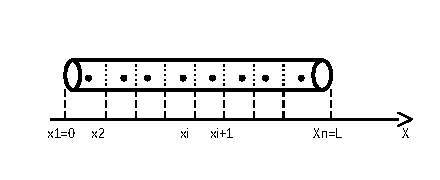
\includegraphics{../img_pdf_cropped/mesh_example}}
    \caption{Пример разбиения непрерывной области - $(0; l)$ на конечное число точек $X(i)$}
    \label{img_mesh_example}
\end{figure}


Для решения задач теплопроводности существует \emph{метод контрольных объёмов}. Подробно этот метод описан в книге \cite{bib:Patankar}. Здесь будут рассмотрены некоторые основные положения как МКО, так и численного решения задач уравнений математической физики в целом. 


Первым отличием численного решения от аналитического является то, что исходная задача заменяется на её аналог, который "<представим"> в ЭВМ. Переходят от непрерывной расчётной области в пространстве к её дискретному аналогу его ещё называют расчётной сеткой. То есть исходная область разделяется на \emph{конечное} число подобластей. Эти подобласти называют контрольными объёмами, в каждом из них выбирается контрольная (узловая, расчётная) точка, она располагается в центре объёма. То же самое относится и ко времени: на заданном непрерывном отрезке времени выбирают промежуточные точки - временные слои. Ставится задача определить значение искомой величины уже в \emph{конечном} наборе точек пространства на каждом временном слое. Итоговым решением является \emph{набор сеточных значений искомой величины}. 


Вторая идея всех численных методов и МКО в частности, состоит в том, что дифференциальное уравнение приводят в вид, который компьютер может обработать. Так как значения искомой величины определяются в заданных точках, то в итоге из исходного ДУ получается система линейных уравнений, по одному уравнению на каждую точку. Уравнения получаются за счёт того, что производные искомой функции определённым образом заменяют на конечные разностные отношения. Этот этап называется дискретизацией уравнения. Получить дискретный аналог ДУ  можно разными способами, всё зависит от того какой вид разностного отношения выбрать для приближения производной. В таких ситуациях чаще всего руководствуются или качественными рассуждениями о протекании процесса, или получают наиболее точное представление математически. Причём бывает так, что для аппроксимации\footnote{Аппроксимация --- приближение} разных (по разным переменным) производных от одной и той же функции используют различные выражения. Поскольку численные методы применяются для нахождения какого-то частного решения задачи, то всегда заранее известны некоторые дополнительные условия. Именно они и позволяют решить полученную систему \emph{линейных} алгебраических уравнений. 


Можно сказать, что метод контрольных объёмов имеет нечто общее с натурными экспериментами. Ведь в них исследователи также обрабатывают результаты измерений полученные в какие-то заданные моменты времени в выбранных точках. Однако \emph{существенная разница здесь в том, что результаты эксперимента представляют собой приближенные измерения реально происходящего процесса, в то время как всякий численный метод в результате отражает некоторую математическую модель.} В случае применения МКО к явлению теплопроводности в твёрдых телах считается, что при достаточно густом разбиении расчётной области все решения сходятся к одной общей величине вне зависимости от выбора способа аппроксимации ДУ. Кроме этого, в данном случае независимая переменная $t$ будет так называемой \emph{односторонней координатой}. Это значит, что величина температуры зависит лишь от того, какой она была на предыдущем временном слое. Поэтому можно последовательно двигаться от одного временного слоя к следующему и так далее, и в итоге определить температуру в нужный момент времени. Это обстоятельство позволяет эффективнее расходовать память при вычислениях. 

\section{Дискретизация расчётной области}
В данной работе сетка будет строиться с равномерным шагом как по координатам, так и по времени. Исходными данными для построения дискретного аналога исследуемой области в одномерном случае будут значения: 
\begin{itemize}
 \item $N_v$ --- Число контрольных объёмов
 \item $l$ --- Длина стержня
 \item $T_{end}$ --- Конечное значение времени
 \item $Nt$ --- Количество временных слоёв
 \label{FVA_defenitions}
\end{itemize}


Пространственная область, т.е. отрезок $[0;\ l]$ разбивается на $N_v$ контрольных объёмов\footnote{Можно считать, что объёмы имеют вид $a\times 1\times 1,$ где $a$ - это расстояние между гранями контрольных объёмов, причём $a \gg 1$.}. В результате можно определить набор значений координат граней контрольных объёмов (в данном случае грани это точки). В каждом контрольном объёме располагается одна узловая точка, в ней определяется значение температуры. На граничные точки тоже приходятся соответствующие узловые точки, чтобы знать температуру границы. Таким образом общее число граней контрольных объёмов $N_f$\footnote{$N_f$ выбрано для обозначения числа граней, от слова "<faces"> - в одном из значений это грань.} равно $N_v + 1$, а узловых точек $N_p$\footnote{$N_p$ индекс $_p$ выбран как сокращение от "<points"> - точки} составляет $N_v + 2$. В МКО предполагается, что каждая узловая точка располагается по середине контрольного объёма. Разбиение временной области тоже делается с равномерным шагом. Его значение можно определить равномерно, например, по конечному времени $T_{end}$ и числу $N_t$, тогда шаг по времени $dt = \frac{T_{end}}{N_t}$. Либо другим способом, для неравномерной стеки. 
\section{Дискретный аналог дифференциального уравнения}
Рассматривается способ получения дискретного аналога следующего уравнения. 
\begin{equation}
\rho c\frac{\partial U(x,t)}{\partial t} \ = \ \frac{\partial}{\partial x}(k\frac{\partial U(x,t)}{\partial x}) \ + \ f(x,t) \label{eq_HeatTransEq_2} 
\end{equation}
\begin{figure}[h!]
 \centering
 \scalebox{2}[1.5]{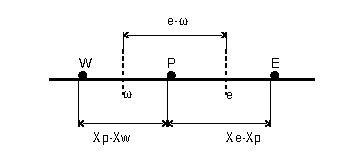
\includegraphics{../img_pdf_cropped/inside_vol}}
 \caption{Изображён типичный внутренний объем с границами $\omega, \ e$ и узловой точкой $p$. \\ Обозначения точек выбраны специально: W "<west"> - западная точка, E "<east"> - восточная. }
 \label{inside_vol}
\end{figure}
\label{integ_diffur}
На рисунке \ref{inside_vol} изображен один из \emph{внутренних} контрольный объёмов. В дальнейшем будет удобно принять обозначения: $T(x) := T(x, t), \ T^0(x) := T(x, t_0)$. Значение температуры во всех узловых точках на предыдущем временном слое считается известными\footnote{Потому что известны начальные условия.}. Уравнение (\ref{commHeatTransEq_2}) можно проинтегрировать в пределах рассматриваемого объёма, то есть при $x \in [\omega, e] $ и за промежуток времени от $t_0$ до $t$. Удобнее начать с левой части уравнения(\ref{commHeatTransEq_2}):
\[
\rho c\frac{\partial T(x, \tau)}{\partial x} \ \Rightarrow \ \rho c\int\limits_{\omega}^e dx \int\limits_{t_0}^t \frac{\partial T(x,\tau)}{\partial x}\ d\tau 
\] 
\\ 
При вычислении внутреннего интеграла $\int\limits_{t_0}^t \frac{\partial T(x,\tau)}{\partial x}\ d\tau$ переменной интегрирования является $\tau$ она принимает множество значений от $t_0$ до $t$. При этом пространственная координата $x$ \emph{фиксированная}. Интегрирование избавляет от производной, поэтому получается выражение: 
\[
\rho c\int\limits_{\omega}^eT(x, \tau)|_{t_0}^t dx \ = \
\rho c\int\limits_{\omega}^e\left(T(x, t) - T(x, t_0)\right) dx
\]
\begin{figure}[b!]
 \subfigure[Вид функции $T(x, t)$ при интегрировании по объёму, когда $t$ - фикс.]{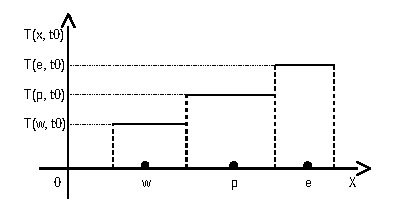
\includegraphics[height=0.22\linewidth,clip]{../img_pdf_cropped/const_func}}
 \hfill
 \subfigure[Вид функции $T(x, t)$ при интегрировании по времени, когда $x$ - фикс.]{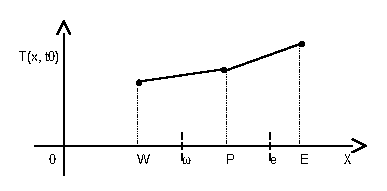
\includegraphics[height=0.22\linewidth,clip]{../img_pdf_cropped/linear_func}}
 \hfill
 \label{func_profiles}
\end{figure}
В полученном выражении стоит разность двух функций от переменной $x$: $T(x, t), \ T(x, t_0)$, где $x \in [\omega; \ e]$. На этом этапе делается предположение, что в \emph{фиксированный момент времени} температура в пределах всего рассматриваемого объёма равна значению температуры в узловой точке $p$. Такая ситуация изображена на рисунке (a). В результате получается:
\[
\rho c\int\limits_{\omega}^e dx \int\limits_{t_0}^t \frac{\partial T(x,\tau)}{\partial x}\ d\tau 
\ = \
\rho c\int\limits_{\omega}^e T(x,\tau)|_{t_0}^t dx  
\ = \ 
\rho c (e - \omega)\left(T(p, t) - T(p, t_0)\right) 
\]
Таким образом, интегрирование левой части (\ref{eq_HeatTransEq_2}) приводит к такому результату:
\begin{equation}
\rho c (e - \omega)\left(T(p) - T^0(p)\right)
\label{eq_integHeatTransLeft1}
\end{equation}
На этапе интегрирования правой части можно, поменять порядок взятия интегралов, так как ~$T(x, t)$ --- непрерывная функция.
\[ 
k \frac{\partial}{\partial x}\left(\frac{T(x, t)}{\partial x}\right) \ \Rightarrow \\ 
k\int\limits_{t_0}^t d\tau \int\limits_{\omega}^e \left(\frac{\partial}{\partial x}(\frac{\partial T(x,\tau)}{\partial x}) + f(x) \right)dx \ 
= 
\]
\[ = 
k\int\limits_{t_0}^t d\tau \int\limits_{\omega}^e \left(\frac{\partial T(x,\tau)}{\partial x}\right)dx + \int\limits_{t_0}^t d\tau \int\limits_{\omega}^e f(x)dx 
\]
Интегрирование первого слагаемого правой части:
\[
k\int\limits_{t_0}^t d\tau \int\limits_{\omega}^e \left(\frac{\partial}{\partial x}(\frac{\partial T(x,\tau)}{\partial x}) \right)dx 
\ = \
k\int\limits_{t_0}^t \left( \frac{\partial T(x,\tau)}{\partial x}\bigg|_{\omega}^e\right) d\tau 
\]
В этом случае изменяться будет значение $x$, то есть значения температуры в фиксированный момент времени в разных точках объёма. На этот раз считается, что в заданный момент времени при переходе от одной точки к другой температура меняется линейно. Это изображено на рис.(b)
%\ref{func_profiles}. 
Поэтому значения производной на границах контрольного объёма можно приблизить разностным отношением температуры в узловых точках в определённый момент времени $\tau$:
\[
\frac{\partial T(e,\tau)}{\partial x} 
\ = \ 
\frac{T(e,\tau) - T(p,\tau)}{x_e - x_p}; \quad \frac{\partial T(\omega,\tau)}{\partial x}
\ = \ 
\frac{T(p,\tau) - T(\omega,\tau)}{x_p - x_{w}}
\]
Первое слагаемое правой части принимает вид:
\[
k\int\limits_{t_0}^t \left( \frac{\partial T(x,\tau)}{\partial x}\bigg|_{\omega}^e\right) d\tau 
 \ = \  
k\int\limits_{t_0}^t \left( \frac{T(e,\tau) - T(p,\tau)}{x_e - x_p} - \frac{T(p,\tau) - T(\omega,\tau)}{x_p - x_{w}} \right) d\tau
\]
\begin{figure}[b!]
 \centering
 \scalebox{2.0}[1.2]{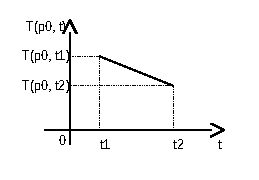
\includegraphics{../img_pdf_cropped/Krank_Nikolson}}
 \caption{Изменение температуры $T$ в фикс. точке $p_0$ за время от $t_0$ до $t$ согласно схеме Кранка-Николсона.}
 \label{img_scemes}
\end{figure}
Получена разность четырех функций от одной переменной - времени. Есть несколько способов решить полученный интеграл. Все они основаны на применении \emph{теоремы о среднем} и различаются предположением о профиле $T(p_0, \tau), p_0$-фикс. Особо известны схемы: явная, неявная, Кранка-Николсона. В данной работе используется схема Кранка-Николсона. Согласно этой схеме температура в фиксированной точке меняется линейно, поэтому средним значением будет среднее арифметическое из значений температуры в моменты $t_0, t$. График изменения температуры в таком случае показан на рис.\ref{img_scemes}. 
Выбор схемы влияет не только на способ решения, но и на требования к сетке. (Подробнее написано в \cite{bib:Patankar}.) Считается, что выбранная схема на равномерной сетке, при соотношении $N_v$ к $N_t$ равном один к одному обеспечивает \emph{второй} порядок точности. Это значит, что когда число объёмов и временных слоёв удваивают, то ошибка решения уменьшается в \emph{четыре} раза. Результат интегрирования правой части:
\[
k\int\limits_{t_0}^t \left( \frac{\partial T(x,\tau)}{\partial x}\bigg|_{\omega}^e\right) d\tau 
\ = \
\frac{k(t - t_0)}{2}\left( \frac{T(e)-T(p)}{x_e - x_p} + \frac{T^0(e)-T^0(p)}{x_e - x_p}\right)
\ - \ 
\]
\begin{equation}
\frac{k(t - t_0)}{2}\left( \frac{T(p)-T(w)}{x_p - x_{w}} + \frac{T^0(p)-T^0(w)}{x_p - x_{w}}\right)
\label{eq_integHeatTransRight1}
\end{equation} \\
Наконец, дошло дело и до второго слагаемого правой части:
\[f(x) \  \Rightarrow \ \int\limits_{t_0}^t d\tau \int\limits_{\omega}^e f(x)dx \]
Так как здесь случай со стационарным источником, то при интегрировании снова можно воспользоваться теоремой о среднем, выбирая постоянное значение $\overline{f_p}$, для данного объёма. Получается выражение вида: \\
\begin{equation}
(t - t_0)(e - \omega)\overline{f_p}
\label{eq_integHeatTransRight2}
\end{equation}
В условии тестовой задачи (на~cтр.\pageref{test_task_page}) известно аналитическое выражение для источникового члена уравнения, поэтому самым лучшим вариантом будет использовать точное выражение интеграла, то есть: \\
\begin{equation}
\int\limits_{t_0}^t d\tau \int\limits_{\omega}^e sin(x)dx 
\ = \ 
\int\limits_{t_0}^t d\tau \left( -cos(e) + cos(\omega) \right) 
\ = \
(t - t_0)\left( -cos(e) + cos(\omega) \right)
\end{equation}
Ранее было сказано, что при переходе от дифференциального уравнения к его дискретному представлению получается система \emph{линейных} уравнений. Как видно сейчас, после интегрирования получаются выражения, содержащие известные значения и искомую величину $T$. Приравнивание результатов интегрирования левой (\ref{eq_integHeatTransLeft1}) и правой частей (\ref{eq_integHeatTransRight1}, \ref{eq_integHeatTransRight2}) уравнения (\ref{eq_HeatTransEq_2}) позволяет выразить температуру в узловой точке данного контрольного объёма. Перед этим удобно сразу разделить обе части на $(t - t_0)$.
\[
\frac{\rho c (e - \omega)}{t - t_0}\left(T(p) - T^0(p)\right) 
\ = \
\frac{k}{2}\left( \frac{T(e)-T(p)}{x_e - x_p} \
+ \frac{T^0(e)-T^0(p)}{x_e - x_p}\right) \ -\]
\[
\ - \
\frac{k}{2}\left( \frac{T(p)-T(w)}{x_p - x_{w}} + \frac{T^0(p)-T^0(w)}{x_p - x_{w}}\right) - cos(e) + cos(\omega) \ \Rightarrow\]
\[ \Rightarrow
\left(\frac{\rho c (e - \omega)}{t - t_0} + \frac{k}{2(x_e - x_p)} + \frac{k}{2(x_p - x_w)} \right)T(p) 
\ = \ \] \\
\begin{equation}
= \ \frac{kT(e)}{2(x_e - x_p)}
\ + \
\frac{kT(w)}{2(x_p - x_w)} 
\ + \
\frac{T^0(e)-T^0(p)}{x_e - x_p}
\ + \
\frac{T^0(p)-T^0(w)}{x_p - x_w} \
 -cos(e) \ + \ cos(\omega)
\label{eq_integHeatTransResult}
\end{equation}
Видно, что в последнем выражении (\ref{eq_integHeatTransResult}) получена зависимость в температуры в точке $p$ от значений её значений в ближайших соседних точках. Для сокращения записей удобно использовать обозначения коэффициентов, как на рис.~\ref{inside_vol}.~со~стр.\pageref{inside_vol}. Буквенные индексы в обозначениях выбраны для удобства восприятия, так $w$ (от англ. "<west">) - западная точка, аналогично $e$ (от англ. "<east">) - восточная точка. \\
\( ae(i) \ = \ \frac{k}{2(x_e - x_p)} \\
 aw(i) \ = \ \frac{k}{2(x_p - x_w)}  \\
 ap(i) \ = \ \frac{\rho c (e - \omega)}{t - t_0} + ae(i) + aw(i)  \\
 bp(i) \ = \ ae(i)\frac{T^0(e)-T^0(p)}{x_e - x_p} - aw(i)\frac{T^0(p)-T^0(w)}{x_p - x_w} + \frac{\rho c (e - \omega)T^0(p)}{t - t_0} -cos(e) + cos(\omega) \)
\\
В итоге получается компактная запись (\ref{eq_insid_vol_Temp}) для уравнения на температуру во \emph{внутренней} точке $p$ на следующем временном слое со значением времени равным $t$. Индексом $i$ нумеруются узловые точки. Левой границе соответствует $i=1$, а правой $i=N_v+2$. (см. обозначения на~стр.\pageref{FVA_defenitions})
\begin{equation}
 ap(i)T(i) \ = \ ae(i)T(i+1) + aw(i)T(i-1) + bp(i), \quad i = \overline{2, n-1}
 \label{eq_insid_vol_Temp}
\end{equation}
Осталось получить выражения для температуры в граничных точках. 
Для левой границы его можно получить из (\ref{eq_integHeatTransResult}): 
\\
\( ap(1)T(1) \ = \ ae(1)T(2) + aw(1)T(0) + bp(1) 
\label{eq_leftBounder_eq} \) \\
Но значения $T(0)$ не существует, поэтому всегда $aw(1) \equiv 0$.
Тогда выражение для температуры на левой границе такое: \\
\(ap(1)T(1) \ = \ ae(1)T(2) + bp(1)\). \\
Аналогично для правой границы: \\
\(ap(n)T(n) \ = \ aw(n)T(n-1) + bp(n)\). \\
Таким образом, получено $N_p$ уравнений для значений температуры в каждой из $N_p$ расчётных точек. Величины $aw(i), ap(i), ae(i)$ и $bp(i)$, где $i=\overline{1, n}$ известны. Поэтому расчёт температуры на следующем временном слое при значении времени равном $t$ сводится к решению системы \emph{линейных} уравнений. 
\section{Решение системы уравнений}
В процессе дискретизации дифференциального уравнения мы получили вот такую систему \emph{линейных} алгебраических уравнений.
\begin{equation} 
\left\{\begin{aligned} 
& ap(1)T(1) \ = \ ae(1)T(2) + bp(1) \\
& ap(2)T(2) \ = \ ae(2)T(3) + aw(2)T(1) + bp(2) \\
& ap(3)T(3) \ = \ ae(3)T(4) + aw(3)T(2) + bp(3) \\
& \dots \\
& ap(n-2)T(n-2) \ = \ ae(n-2)T(n-1) + aw(n-2)T(n-3) + bp(n-2) \\
& ap(n)T(n) \ = \ aw(n)T(n-1) + bp(n) 
\end{aligned}\right.
\label{eq_SLAU}
\end{equation}
Видно, что её матрица довольно своеобразная. Ненулевые значения сконцентрированы рядом с главной диагональю. Существует \emph{прямой} метод решения СЛАУ такого вида. У его принято называть методом \emph{прогонки}\footnote{В иностранной литературе из-за трёхдиагонального вида матрицы этот алгоритм называется TDMA}.
Из первого уравнения системы (\ref{eq_SLAU}) видно, что значение $T(1)$ можно выразить через $T(2)$. То есть:\\
\( ap(1)T(1) \ = \ ae(1)T(2) + bp(1) \Rightarrow \\ 
T(1) = \frac{ae(1)T(2)}{ap(1)} + \frac{bp(1)}{ap(1)} \ = \ P(1)T(2) + Q(1), \quad P(1)\ = \ \frac{ae(1)}{ap(1)}, \quad Q(1) \ = \ \frac{bp(1)}{ap(1)}\)  \\
Из второго уравнения температура $T(2)$ определяется значениями в соседних точках $T(1), \ T(3)$, но можно $T(1)$ представить через $T(2)$. Связь $T(1)$ и $T(2)$ даёт следующее: \\
\( ap(2)T(2) \ = \ ae(2)T(3) + aw(2)T(1) + bp(2) \ = \ aw(2)\left(P(1)T(2) + Q(1) \right) + bp(2) \Rightarrow  \\
\left(ap(2) - aw(2)P(1)\right)T(2) \ = \ ae(2)T(3) + aw(2)Q(1) + bp(2) \Rightarrow \\
T(2) \ = \ P(2)T(3) + Q(2) \ \), где $P(2) \ = \ \frac{ae(2)}{ap(2) - aw(2)P(1)}, \ Q(2) \ = \ \frac{aw(2)Q(1) + bp(2)}{ap(2) - aw(2)P(1)}$ \\
Ясно, что продолжая такие же рассуждения можно получить зависимость температуры 
\begin{equation}
T(i) от T(i+1 в виде T(i) = P(i)T(i+1) + Q(i) 
\label{eq_TDMA_Ti_1}
\end{equation}
Уравнение выше позволяет выразить температуру $T(i)$ для\emph{каждой внутренней} точки $i=\overline{2=n-1}$ температуру справа, то есть $T(i+1)$. \\
С другой стороны известно представление $T(i)$ в виде, вкотором оно записано в системе (\ref{eq_SLAU}) \\
$ap(i)T(i) \ = \ ae(i)T(i+1) + aw(i)T(i-1) + bp(i)$ \\
В последнем уравнении можно исключить $T(i-1)$ \\
\( ap(i)T(i) \ = \ ae(i)T(i+1) + aw(i)\left(P(i-1)T(i)+Q(i-1)\right) + bp(i) \Rightarrow \\
\left(ap(i) - aw(i)P(i-1)\right)T(i) \ = \ ae(i)T(i+1) + aw(i)Q(i-1) + bp(i) \Rightarrow \\ \)
\begin{equation}
\Rightarrow \ T(i) = \frac{ae(i)T(i+1)}{ap(i) - aw(i)P(i-1)} + \frac{aw(i)Q(i-1) + bp(i)}{ap(i) - aw(i)P(i-1)}
\label{eq_TDMA_Ti_2}
\end{equation}
\\
Для температуры $T(i)$ найдено два представления, значит из (\ref{eq_TDMA_Ti_2}) можно найти формулы для коэффициентов $P(i), Q(i)$ в (\ref{eq_TDMA_Ti_1}) при $i=\overline{2,n-1}$ \\
В этом состоит первая часть алгоритма прогонки --- прямой ход, когда вычисляются коэффициенты $P(i), Q(i)$. Но решить выражение не получается, так как неизвестно значение $T(i+1)$. В общем случае, при численном решении уравнения теплопроводности после того, как выполнен этап прямого хода значение $T(n)$. В случае для \emph{первой} начально-краевой задачи, получается, что известны значения температуры на границах. Тестовая задача (\ref{test_task}, стр.(\pageref{test_task_page})) однородная, что означает $T(n) \Rightarrow ap(n) = P(n) = Q(n) = 0$. Теперь, можно найти значение $T(n-1)$, через него получается $T(n-2)$ ну и так далее до $T(2)$, а значение $T(1)$ задано из граничных условий. Такая процедура называется \emph{обратным} ходом и с её помощью вычисляются значения температуры в каждой узловой точке \emph{одного} временного слоя. Всего временных слоёв $N_t$.

\section{Алгоритм метода прогонки}
\begin{enumerate}
 \item Пользуясь граничными условиями, вычислить: $P(1), \ Q(1)$.
 \item Прямой ход --- определение величин: \\ \(P(i) = \frac{ae(i)}{ap(i) - aw(i)P(i-1)}, \quad Q(i) = \frac{aw(i)Q(i-1) + bp(i)}{ap(i) - aw(i)P(i-1)}\)
 \item Получить значение $T(N)$, используя граничные условия. 
 \item Выполнить обратный ход, находя $T(i)$ по формуле: \\ $T(i) \ = \ P(i)T(i+1) \ + \ Q(i)$
\end{enumerate}

\chapter{Описание программной реализации МКО}
\section{Общая схема программы}
\begin{figure}[hb!]
 \centering{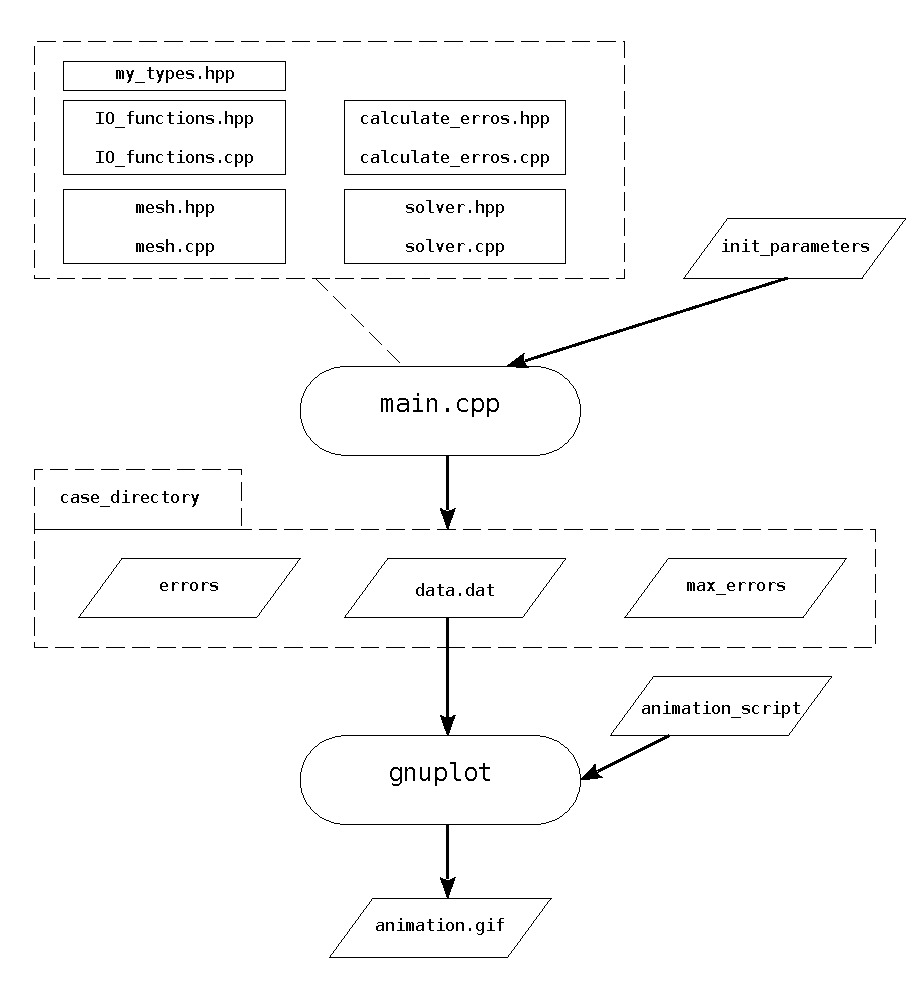
\includegraphics{../img_pdf_cropped/prog_scheme}}
 \caption{Структура вычислительной программы, её взаимодействие с утилитой gnuplot.}
 \label{prog_scheme}
\end{figure}
\newpage
Описание взаимодействия пользователя с программой. Для того, чтобы провести расчёт первой начально-краевой задачи, нужно передать входные данные. Это делается с помощью текстового файла. В файле необходимо перечислить параметры задачи в ~\emph{соответствии со следующим форматом:}
\begin{itemize}
 \item "<значение длины">
 \item "<количество контрольных объёмов">
 \item "<конечное время">
 \item "<число временных слоёв">
 \item "<плотность материала">
 \item "<удельная теплоёмкость">
 \item "<коэффициент теплопроводности">
\end{itemize}

При этом, для удобства в начале каждой строки можно подписать, какой именно параметр в ней записан, например $\rho = 1000$ --- допустимая запись. После этого нужно вызвать исполняемый файл программы передав ей в качестве первого аргумента имя файла с исходными данными, а вторым аргументом ввести имя директории, где будут сохранены результаты расчётов. Для визуализации вычислений  используется свободно распространяемая программа gnuplot. Специально для создания анимаций на основе расчётных данных был создан специальный скрипт\footnote{скрипт - в данном случае это файл с заготовленным набором команд для программы gnuplot.} для gnuplot. По задумке этот скрипт поставляется вместе с вычисляющей программой. Поэтому пользователю, находящемуся в каталоге с результатами расчётов, нужно лишь перенаправить в gnuplot команды из скрипта. Это делается очень просто: вызывается gnuplot и аргументом указывается имя скрипта. В итог будет сформирован файл с анимацией в формате "<.gif">. Для изменения параметров анимации нужно всего лишь отредактировать нужные поля в текстовом файле скрипта. Теперь, когда ясно как с этим \emph{работать,} нужно объяснить как это \emph{работает.} 


Вся расчётная программа написана на языке C++ с использованием стандартных библиотек языков C и C++. Выбор этого языка объсяется тем, что C++ хорошо подходит для расчётов, благодаря своей быстроте. Он позволяет создавать достаточно оптимизированные программы, так как в нём есть возможность прямого контроля памяти. В данном случае эффективное взаимодействие с памятью имеет значение. Поскольку для представления дискретных наборов значений хорошо подходят массивы, то они и применяются для представления расчётной сетки, набора значений численного и эталонного решений, величин погрешностей. Но \emph{пользователь может указывать разное} число расчётных точек, поэтому статические массивы не пригодны. В созданной программе память под все массивы выделяется \emph{динамически.} А C++ позволяет напрямую контролировать этот процесс: выделять ровно столько, сколько нужно, и освобождать память, как только она больше не нужна. 
\label{page_model_user}
С самого начала было решено, что программа будет состоять из модулей. В верхней части схемы на странице \pageref{prog_scheme} в пунктирной рамке изображены 5 модулей, которые подключаются к модулю "<\texttt{main}">, содержащему главную функию. В самом первом модуле "<\texttt{my\_types}"> описаны структуры данных, которые используются при ведении вычислений. Объединение нескольких базовых типов данных в один составной - структуру позволяет сократить объём кода, а также сделать его восприятие более доступным.


Основное удобство представления программы в виде нескольких обособленных частей состоит в том, что в этом случае существенно упрощается модернизация программы, а следовательно, расширяются её возможности. Например, если будет решено сделать неравномерную расчётную сетку, то потребуется лишь изменить содержимое модуля "<\texttt{mesh}">\footnote{от англ. \emph{mesh} - сеть}, а лучше сделать две версии и в разных ситуациях использовать наиболее подходящую. Кроме этого в таком формате код лучше воспринимается, ведь каждый модуль отвечает за конкретную задачу. Если код программы большой, то неудобно просматривать его. А когда программа разбита на модули, то программисту нужно смотреть лишь код интересующего его модуля, что заметно проще. Нужно отметить, что модуль может состоять как из одного, так и из двух файлов. Если в модуле реализованы функции, которые будут использовать другими частями программы вне его, то синтаксис языка C++ требует, объявления этих переменных в тех частях программы, где они используются, а их реализации могут располагаться в другом файле. В этой программе "<парных модулей четыре">. \\
Краткое описание предназначения модулей.
\begin{itemize}
 \item "<\texttt{my\_types}"> --- В нём введены новые структуры данных, представляющие: сетку, физические константы, массивы с погрешностями.
 \item "<\texttt{IO\_functions}"> --- Этот модуль отвечает за обработку файла с исходными данными задачи, а также вывод результатов работы программы.
 \item "<\texttt{mesh}"> --- В нём реализованы функции для создания равномерной расчётной сетки.
 \item "<\texttt{solver}"> --- В данном модуле реализован алгоритм\footnote{Имеется ввиду описанный выше алгоритм ТДМА.} решения системы уравнений, которая позволяет определить температуру на следующем временном слое. 
 \item "<\texttt{calculate\_errors}"> --- Эта часть программы отвечает за вычисление абсолютных и относительных погрешностей. После этапа тестирования её можно не подключать.
 \item "<\texttt{main}"> --- "<Главная подпрограмма"> в ней происходит вызов функций из всех остальных функций, описанных в подключаемых модулях. 
\end{itemize}
\newpage
\section{Модуль "<\texttt{my\_types}">}
\large
\listinginput{1}{../program/my_types.hpp}
\Large
Далее будет приведён исходный код каждого модуля, а также скрипта для анимации. Поясняющие комментарии написаны прямо в коде. 
\section{Модуль "<\texttt{IO\_functions}">}
\large
\listinginput{1}{../program/IO_functions.hpp}
\listinginput{1}{../program/IO_functions.cpp}
\Large
\section{Модуль "<\texttt{mesh}">}
\large 
\listinginput{1}{../program/mesh.hpp}
\listinginput{1}{../program/mesh.cpp}
\Large
\section{Модуль "<\texttt{solver}">}
Пожалуй самый "<интересный"> из всех модулей. Собственно в нём реализован метод решения системы линейных уравнений, решение которой даёт значения температуры. В данной программе вычислительная часть настроена на решение задачи с нулевыми граничными условиями первого рода. Но можно изменить несколько строк когда, где вычисляется прогоночные коэффициенты и получится, что программа способна решать и \emph{ненулевые} первые начально-краевые задачи.Ниже приведён код заголовочного файла модуля "<\texttt{solver}">.
\large 
\listinginput{1}{../program/solver.hpp}
\Large 
Далее идёт листинг с исходным файлом данного модуля. Нужно сказать, что при необходимости максимально ускорить вычисления данную версию решателя можно переделать. Сейчас при вычислениях в нескольких местах локальным переменным переприсваиваются те же самые данные, что и в структуре \texttt{mesh}. Это сделано для того, чтобы упростить восприятие кода. 
\large
\listinginput{1}{../program/solver.cpp}
\Large
\section{Модуль "<\texttt{calculate\_errors}">}
\large
\listinginput{1}{../program/calculate_errors.hpp}
\listinginput{1}{../program/calculate_errors.cpp}
\Large
\section{Модуль "<\texttt{main}">}
Главная функция "<\texttt{main}"> вызывает большинство процедур из описанных выше модулей. В ней подготавливается директория для сохранения файлов с данными расчётов и инициализируются нужные структуры данных. Потом запускается расчётный цикл, в котором вызывается процедура "<\texttt{TDMA}">\footnote{Код программы написан с учётом того, что его может посмотреть иностранный программист. Поэтому название выбрано от слов Tridiagonal matrix algorithm.}, итерации идут для каждого временного слоя. На каждой итерации происходит расчёт температуры в узловых точках на текущем временном слое, вывод расчётных значений и погрешностей в соответствующие файлы. Ниже приведён исходный код.
\large
\listinginput{1}{../program/main.cpp}
\Large

\section{Скрипт для визуализации результатов расчётов в gnuplot}
Утилита gnuplot поддерживает два режима работы. Один из них это выполнение команд из заданного файл. Это и применяется для построения анимации по результатам расчётов. При необходимости можно изменить настройки анимации, например, изменив задержку между кадрами или цвет графика. 
\large
\listinginput{1}{../program/AnimatioScript}
\Large

\newpage
\def \hfillx {\hspace*{-\textwidth} \hfill}
\begin{table}[th!]
\centering
\section{Результаты тестирования}
\begin{minipage}{0.3\textwidth}
\centering
\caption{\\ Число контрольных объёмов - 5.\\Число временных слоёв - 5.}
\begin{tabular}{|c|c|c|}
\hline \multicolumn{3}{|c|}{ погрешность} \\
\hline 
время сек. & абс. & относ. в \%
\\
\hline 
0.200 & 0.001898 & 3.289 \\
0.400 & 0.002584 & 2.463 \\
0.600 & 0.002432 & 1.694 \\
0.800 & 0.001720 & 0.981 \\
1.000 & 0.000652 & 0.324 \\
\hline
\end{tabular}
%
%
%
\end{minipage}
\hfillx
\begin{minipage}{0.3\textwidth}
\centering
\caption{\\ Число контрольных объёмов - 10. \\ Число временных слоёв - 10.}
\begin{tabular}{|c|c|c|}
\hline \multicolumn{3}{|c|}{ погрешность} \\
\hline 
время сек. & абс. & относ. в \%
\\
\hline 
0.100 & 0.000275 & 0.908 \\
0.200 & 0.000462 & 0.800 \\
0.300 & 0.000573 & 0.695 \\
0.400 & 0.000623 & 0.594 \\
0.500 & 0.000622 & 0.497 \\
0.600 & 0.000579 & 0.403 \\
0.700 & 0.000501 & 0.313 \\
0.800 & 0.000397 & 0.226 \\
0.900 & 0.000271 & 0.144 \\
1.000 & 0.000129 & 0.064 \\
\hline
\end{tabular}
\end{minipage}
\hfillx
%
%
\begin{minipage}{0.3\textwidth}
\centering
\caption{\\ Число контрольных объёмов - 20. \\ Число временных слоёв - 20.}
\begin{tabular}{|c|c|c|}
\hline \multicolumn{3}{|c|}{ погрешность} \\
\hline 
время сек. & абс. & относ. в \%
\\
\hline 
0.050 & 0.000038 & 0.243 \\
0.100 & 0.000069 & 0.229 \\
0.150 & 0.000095 & 0.215 \\
0.200 & 0.000116 & 0.201 \\
0.250 & 0.000132 & 0.188 \\
0.300 & 0.000144 & 0.175 \\
0.350 & 0.000152 & 0.162 \\
0.400 & 0.000156 & 0.149 \\
0.450 & 0.000158 & 0.137 \\
0.500 & 0.000156 & 0.124 \\
0.550 & 0.000151 & 0.112 \\
0.600 & 0.000145 & 0.101 \\
0.650 & 0.000136 & 0.089 \\
0.700 & 0.000125 & 0.078 \\
0.750 & 0.000112 & 0.067 \\
0.800 & 0.000098 & 0.056 \\
0.850 & 0.000083 & 0.046 \\
0.900 & 0.000066 & 0.035 \\
0.950 & 0.000049 & 0.025 \\
1.000 & 0.000030 & 0.015 \\
\hline
\end{tabular}
\end{minipage}
\end{table}

Когда производилось интегрирование уравнения (на~стр.\pageref{integ_diffur}) было сказано, что существует несколько подходов при интегрировании по времени. Была выбрана схема Кранка-Николсона. Согласно теоретическим рассуждениям, при её использовании должен быть \emph{второй} порядок точности. Это означает, что при \emph{удвоении} числа расчётных точек ошибка должна уменьшаться в \emph{четыре} раза. Выше приведены таблицы. Один из столбцов содержит абсолютные погрешности, в а другой относительные. В этих таблицах в записаны \emph{наибольшие} значения соответствующих погрешностей среди \emph{всех узловых точек} для каждого временного слоя, значение времени указано в первом столбце. Ошибки вычислялись при сравнении температуры, посчитанной программой с точным значением, которое определяется решением задачи на (стр.~\pageref{test_task_page}).

Нужно уточнить, что для вычисления абсолютной погрешности использовалась стандартная формула: $\Delta T = |T^{*} - T_{т}|$, а для относительной погрешности $\delta T$ значение в знаменателе было заменено на \emph{среднее} по всему временному слою. Среднее значение~$\overline{T}$ определялось интегрированием: $\overline{T}\ =\ \frac{1}{\pi}\int\limits_{0}^{pi}\ T(x, t_0) dx$. И итоговая формула для относительной погрешности, которая реализована в коде такая: $\frac{|T - T^{*}|}{\overline{T}}$ 

Результаты, представленные в таблицах подтверждают хорошую точность приближенного вычисления температуры на основании численного метода - метода контрольных объёмов. Кроме того, видно, что соблюдается выполнение второго порядка точности. Таким образом, при реализации процедуры разбиения расчётной области и вычислительного алгоритма ошибок нет.

\chapter{Заключение}
В ходе работы была проведена теоретическая подготовка. Изучена математическая модель описываемого процесса теплопроводности, а также численный метод решения задач из этой области --- метод контрольных объёмов. В ходе работы удалось реализовать этот метод решения в виде расчётной программы, состоящей из нескольких частей. Результаты тестирования подтвердили теоретический прогноз о том, что схема Кранка-Николсона даёт второй порядок точности. В результате появился первый опыт компьютерного моделирования. Также удалось развить навыки программирования, так как в при создании программы в этом проекте активно использовалась раздельная сборка программы, работа с файлами, взаимодействие нескольких программ. Во время работы на программой часто помогала информация из \cite{bib:Stolyarov}. Для разработки программы был выбран модульный подход. Это позволит с лёгкостью модернизировать начальную версию. Выходные данные создаваемые в процессе вычисления программой сделаны в формате, который поддерживается свободно распространяемой программой gnuplot, это позволяет визуализировать результаты расчётов. Модель взаимодействия конечного пользователя с программой, подробно описанная на (стр. \pageref{page_model_user}) подходит к использованию даже тем людям, кто не владеет навыками программирования. 
\bibliographystyle{ugost2008}
\bibliography{bibliography}
\end{document}
